%! Author = Len Washington III
%! Date = 9/12/2023

% Preamble
\documentclass[12pt]{report}

% Packages
\usepackage[12]{cs430lecture}

% Document
\begin{document}

%<*Lecture-Activity-12>
\section{Opening Questions}\label{sec:opening-questions-12}
\begin{enumerate}[label=\arabic*.]
    \item What do you think the issue we need to handle when deleting a node from a red-black tree? How does red-black delete differ from a \hyperref[alg:bst-delete]{BST delete}? \answer{If the actaul node deleted is red, then you're done. If the node you're deleting is black, then you potentially could have two red nodes in a row. If you color the deleted nodes child black (if it was red), then you're done. There would only be 0 or 1 children, not 2. If the child was already black, you add an extra ``blackness'' to temporarily fix the black-height problem, meaning the node counts for 2 black nodes.}
\end{enumerate}

\section{Red-Black Tree Delete}\label{sec:red-black-tree-delete}
\begin{itemize}
    \item Think of $V$ as having an ``extra'' unit of blackness. This extra blackness must be absorbed into the tree (by a red node), or propagated up to the root and out of the tree. There are four cases -- our examples and ``rules'' assume that $V$ is a left child. There are symmetric cases for $V$ as a right child
\end{itemize}

Terminology in Examples
\begin{itemize}
    \item The node just deleted was $U$
    \item The node that replaces it is $V$, which has an extra unit of blackness
    \item The parent of $V$ is $P$
    \item The sibling of $V$ is $S$
\end{itemize}
\begin{figure}[H]
    \centering
    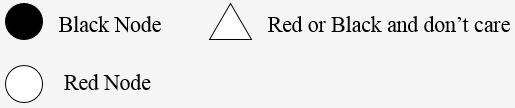
\includegraphics[width=\textwidth]{12.1}
    \caption{Red Black Tree Graphics Definitions}
    \label{fig:12.1}
\end{figure}

\begin{minipage}{0.475\textwidth}
    \begin{itemize}
        \item $V$'s sibling, $S$ is Red
        \begin{itemize}
            \item Rotate $S$ around $P$ and recolor $S$ \& $P$
        \end{itemize}
        \item NOT a terminal case -- One of the other cases with now apply
        \item All other cases apply when $S$ is Black
    \end{itemize}
\end{minipage}\hfill
\begin{minipage}{0.5\textwidth}
    \begin{figure}[H]
        \centering
        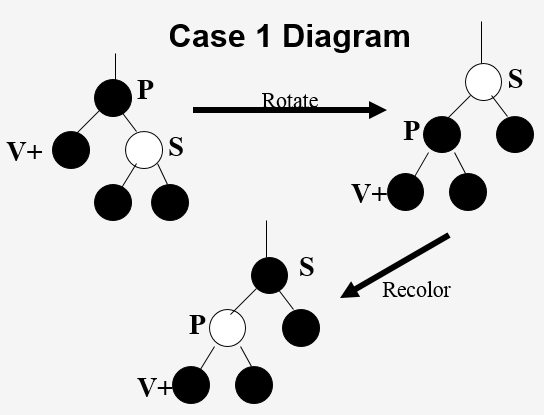
\includegraphics[width=\textwidth]{12.2}
        \caption{Red Black Tree Delete Case \#1}
        \label{fig:red-black-delete-case-1}
    \end{figure}
\end{minipage}\\
\begin{minipage}{0.475\textwidth}
    \begin{itemize}
        \item $V$'s sibling, $S$ is black and has \emph{two black children.}
        \begin{itemize}
            \item Recolor $S$ to be Red
            \item $P$ absorbs $V$'s extra blackness
            \begin{itemize}
                \item If $P$ was Red, make it black, we're done
                \item If $P$ was Black, it now has extra blackness and problem has been propagated up the tree
            \end{itemize}
        \end{itemize}
    \end{itemize}
\end{minipage}\hfill
\begin{minipage}{0.5\textwidth}
    \begin{figure}[H]
        \centering
        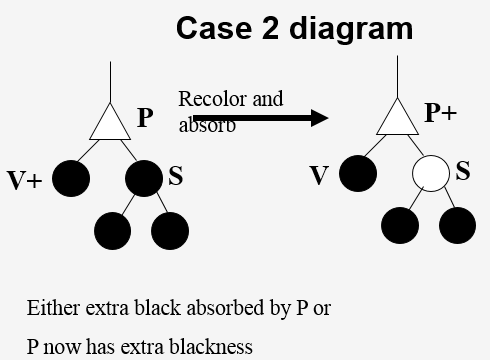
\includegraphics[width=\textwidth]{12.3}
        \caption{Red Black Tree Delete Case \#2}
        \label{fig:red-black-delete-case-2}
    \end{figure}
\end{minipage}\\
\begin{minipage}{0.475\textwidth}
    \begin{itemize}
        \item $S$ is black
        \item $S$'s RIGHT child is RED (Left child either color)
        \begin{itemize}
            \item Rotate $S$ around $P$
            \item Swap colors of $S$ and $P$, and color $S$'s Right child Black
        \end{itemize}
        \item This is the terminal case -- we're done
    \end{itemize}
\end{minipage}\hfill
\begin{minipage}{0.5\textwidth}
    \begin{figure}[H]
        \centering
        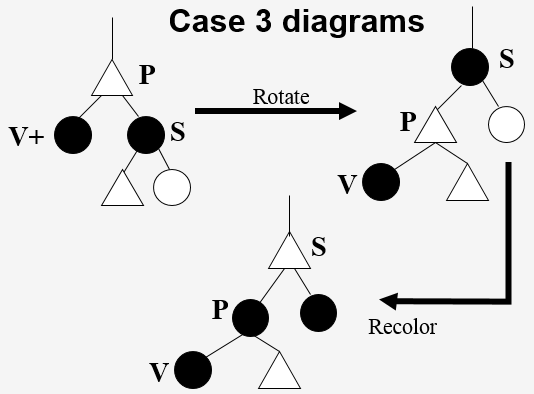
\includegraphics[width=\textwidth]{12.4}
        \caption{Red Black Tree Delete Case \#3}
        \label{fig:red-black-delete-case-3}
    \end{figure}
\end{minipage}\\
\begin{minipage}{0.475\textwidth}
    \begin{itemize}
        \item $S$ is Black, $S$'s right child is Black and $S$'s left child is Red
        \begin{itemize}
            \item Rotate $S$'s left child around $S$
            \item Swap color of $S$ and $S$'s left child
            \item Now in \hyperref[fig:red-black-delete-case-3]{case 3}
        \end{itemize}
    \end{itemize}
\end{minipage}\hfill
\begin{minipage}{0.5\textwidth}
    \begin{figure}[H]
        \centering
        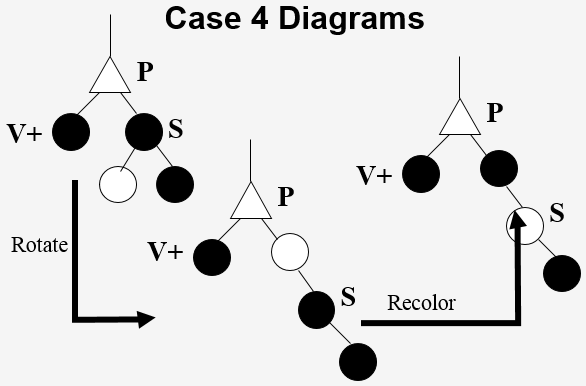
\includegraphics[width=\textwidth]{12.5}
        \caption{Red Black Tree Delete Case \#4}
        \label{fig:red-black-delete-case-4}
    \end{figure}
\end{minipage}

Red Black Visualization:
\begin{itemize}
    \item \url{http://gauss.ececs.uc.edu/RedBlack/redblack.html}
    \item \url{https://www.cs.usfca.edu/~galles/visualization/RedBlack.html}
\end{itemize}

\section{AVL Trees}\label{sec:avl-trees}
An AVL tree is a special type of binary tree that is always ``partially'' balanced. The criteria that is used to determine the ``level'' of ``balanced-ness'' is the difference between the heights of sub-trees of every node in the tree. The ``height'' of the tree is the ``number of levels'' in the tree.

AN AVL tree is a special binary tree in which the difference between the height of the right and left sub-trees (of any node) is never more than one.
\begin{enumerate}[label=\arabic*.]
    \item How do you think we could keep track of the height of the right and left sub-trees of every node?
    \item If we find an imbalance, how can we correct it without adding any significant cost to the insert of delete?
\end{enumerate}

\begin{minipage}{0.475\textwidth}
    Single Rotations\\The imbalance is left-left (or right-right)
    \begin{figure}[H]
        \centering
        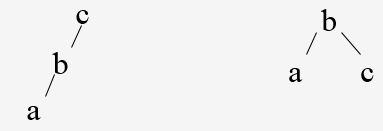
\includegraphics[width=\textwidth]{12.6}
        \label{fig:12.6}
    \end{figure}
    Perform single right rotation at $c$ (R-rotation)\\Similar idea for single left rotation (L-rotation)
\end{minipage}\hfill
\begin{minipage}{0.5\textwidth}
    Double Rotations\\The imbalance is left-right (or right-left)
    \begin{figure}[H]
        \centering
        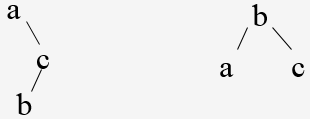
\includegraphics[width=\textwidth]{12.7}
        \label{fig:12.7}
    \end{figure}
    Perform right rotation at $c$ then left rotation at $a$ (RL-rotation)\\Similar idea for left rotation then right rotation (LR-Rotation)
\end{minipage}

~\\\vspace*{2em}AVL Visualization: \url{https://visualgo.net/bn/bst}
%</Lecture-Activity-12>

\end{document}